\section{tasks::autoload Class Reference}
\label{classtasks_1_1autoload}\index{tasks::autoload@{tasks::autoload}}
Inheritance diagram for tasks::autoload::\begin{figure}[H]
\begin{center}
\leavevmode
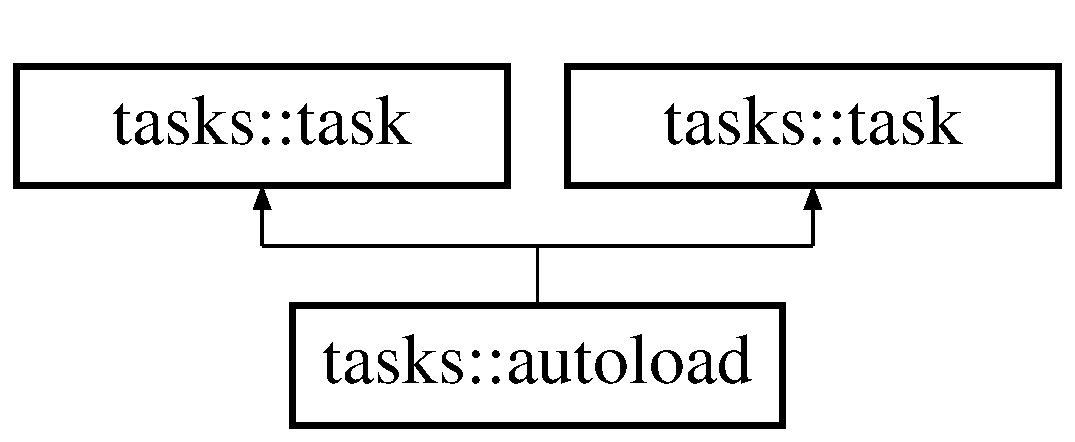
\includegraphics[height=2cm]{classtasks_1_1autoload}
\end{center}
\end{figure}
\subsection*{Public Member Functions}
\begin{CompactItemize}
\item 
def \textbf{run}\label{classtasks_1_1autoload_cbc6ebe4d736fc571c9e08024c68b88b}

\item 
def \textbf{run}\label{classtasks_1_1autoload_cbc6ebe4d736fc571c9e08024c68b88b}

\end{CompactItemize}
\subsection*{Static Public Attributes}
\begin{CompactItemize}
\item 
string \textbf{name} = '{\bfautoload}'\label{classtasks_1_1autoload_1141ed7ffd19b60ebecbc0b7bc699800}

\item 
string \textbf{button\-Text} = 'Auto\-Load configuration'\label{classtasks_1_1autoload_5e7ed731bc97b0437792affe7a10279a}

\end{CompactItemize}


\subsection{Detailed Description}


\footnotesize\begin{verbatim}Automatically load a pipeline configuration depending on
   the values of FITS headers. This is useful when processing a set
   of frames with different settings for binning or windowing
\end{verbatim}
\normalsize
 



The documentation for this class was generated from the following files:\begin{CompactItemize}
\item 
old/PANICtool-1.0/tasks.py\item 
old/tasks.py\end{CompactItemize}
